% This file does not have the appropriate header and tags to compile in latex. It is meant to be input into another file for compiling. 
% This document is based on electronic transcriptions by Joseph Ransdell and Brian Kariger, which used to be available at the Arisbe website: http://www.iupui.edu/~arisbe/

\section*{How to Make Our Ideas Clear}
\emph{This is the sequel to ``The Fixation of Belief'' and can be read as a continuation of the same argument. It was originally published in \emph{Popular Science Monthly} 12 (January 1878), pgs. 286--302.}

\subsection*{I}

Whoever has looked into a modern treatise on logic of the common sort, will doubtless remember the two distinctions between \emph{clear} and \emph{obscure} conceptions, and between \emph{distinct} and \emph{confused} conceptions. They have lain in the books now for nigh two centuries, unimproved and unmodified, and are generally reckoned by logicians as among the gems of their doctrine.


A clear idea is defined as one which is so apprehended that it will be recognized wherever it is met with, and so that no other will be mistaken for it. If it fails of this clearness, it is said to be obscure.


This is rather a neat bit of philosophical terminology; yet, since it is clearness that they were defining, I wish the logicians had made their definition a little more plain. Never to fail to recognize an idea, and under no circumstances to mistake another for it, let it come in how recondite a form it may, would indeed imply such prodigious force and clearness of intellect as is seldom met with in this world. On the other hand, merely to have such an acquaintance with the idea as to have become familiar with it, and to have lost all hesitancy in recognizing it in ordinary cases, hardly seems to deserve the name of clearness of apprehension, since after all it only amounts to a subjective feeling of mastery which may be entirely mistaken. I take it, however, that when the logicians speak of ``clearness,'' they mean nothing more than such a familiarity with an idea, since they regard the quality as but a small merit, which needs to be supplemented by another, which they call \emph{distinctness.}

A distinct idea is defined as one which contains nothing which is not clear. This is technical language; by the \emph{contents} of an idea logicians understand whatever is contained in its definition. So that an idea is \emph{distinctly} apprehended, according to them, when we can give a precise definition of it, in abstract terms. Here the professional logicians leave the subject; and I would not have troubled the reader with what they have to say, if it were not such a striking example of how they have been slumbering through ages of intellectual activity, listlessly disregarding the enginery of modern thought, and never dreaming of applying its lessons to the improvement of logic. It is easy to show that the doctrine that familiar use and abstract distinctness make the perfection of apprehension has its only true place in philosophies which have long been extinct; and it is now time to formulate the method of attaining to a more perfect clearness of thought, such as we see and admire in the thinkers of our own time.

When Descartes set about the reconstruction of philosophy, his first step was to (theoretically) permit scepticism and to discard the practice of the schoolmen of looking to authority as the ultimate source of truth. That done, he sought a more natural fountain of true  principles, and thought he found it in the human mind; thus passing, in the directest way, from the method of authority to that of apriority, as described in my first paper. Self-consciousness was to furnish us with our fundamental truths, and to decide what was agreeable to reason. But since, evidently, not all ideas are true, he was led to note, as the first condition of infallibility, that they must be clear. The distinction between an idea \emph{seeming} clear and really being so, never occurred to him.  Trusting to introspection, as he did, even for a knowledge of external things, why should he question its testimony in respect to the contents of our own minds? But then, I suppose, seeing men, who seemed to be quite clear and positive, holding opposite opinions upon fundamental principles, he was further led to say that clearness of ideas is not sufficient, but that they need also to be distinct, i.e., to have nothing unclear about them. What he probably meant by this (for he did not explain himself with precision) was, that they must sustain the test of dialectical examination; that they must not only seem clear at the outset, but that discussion must never be able to bring to light points of obscurity connected with them.


Such was the distinction of Descartes, and one sees that it was precisely on the level of his philosophy. It was somewhat developed by Leibnitz. This great and singular genius was as remarkable for what he failed to see as for what he saw. That a piece of mechanism could not do work perpetually without being fed with power in some form, was a thing perfectly apparent to him; yet he did not understand that the machinery of the mind can only transform knowledge, but never originate it, unless it be fed with facts of observation. He thus missed the most essential point of the Cartesian philosophy, which is, that to accept propositions which seem perfectly evident to us is a thing which, whether it be logical or illogical, we cannot help doing. Instead of regarding the matter in this way, he sought to reduce the first principles of science to two classes, those which cannot be denied without self-contradiction, and those which result from the principle of sufficient reason (of which more anon), and was apparently unaware of the great difference between his position and that of Descartes. So he reverted to the old trivialities of logic; and, above all, abstract definitions played a great part in his philosophy. It was quite natural, therefore, that on observing that the method of Descartes labored under the difficulty that we may seem to ourselves to have clear apprehensions of ideas which in truth are very hazy, no better remedy occurred to him than to require an abstract definition of every important term. Accordingly, in adopting the distinction of \emph{clear} and \emph{distinct} notions, he described the latter quality as the clear apprehension of everything contained in the definition; and the books have ever since copied his words. There is no danger that his chimerical scheme will ever again be over-valued. Nothing new can ever be learned by analyzing definitions. Nevertheless, our existing  beliefs can be set in order by this process, and order is an essential element of intellectual economy, as of every other. It may be acknowledged, therefore, that the books are right in making familiarity with a notion the first step toward clearness of apprehension, and the defining of it the second. But in omitting all mention of any higher perspicuity of thought, they simply mirror a philosophy which was exploded a hundred years ago. That much-admired ``ornament of logic''--- the doctrine of clearness and distinctness--- may be pretty enough, but it is high time to relegate to our cabinet of curiosities the antique \emph{bijou,} and to wear about us something better adapted to modern uses.

The very first lesson that we have a right to demand that logic shall teach us is, how to make our ideas clear; and a most important one it is, depreciated only by minds who stand in need of it. To know what we think, to be masters of our own meaning, will make a solid foundation for great and weighty thought. It is most easily learned by those whose ideas are meagre and restricted; and far happier they than such as wallow helplessly in a rich mud of conceptions. A nation, it is true, may, in the course of generations, overcome the disadvantage of an excessive wealth of language and its natural concomitant, a vast, unfathomable deep of ideas. We may see it in history, slowly perfecting its literary forms, sloughing at length its metaphysics, and, by virtue of the untirable patience which is often a compensation, attaining great excellence in every branch of mental acquirement. The page of history is not yet unrolled that is to tell us whether such a people will or will not in the long run prevail over one whose ideas (like the words of their language) are few, but which  possesses a wonderful mastery over those which it has. For an individual, however, there can be no question that a few clear ideas are worth more than many confused ones. A young man would hardly be persuaded to sacrifice the greater part of his thoughts to save the rest; and the muddled head is the least apt to see the necessity of such a sacrifice. Him we can usually only commiserate, as a person with a congenital defect. Time will help him, but intellectual maturity with regard to clearness comes rather late, an unfortunate arrangement of Nature, inasmuch as clearness is of less use to a man settled in life, whose  errors have in great measure had their effect, than it would be to one whose path lay before him. It is terrible to see how a single unclear idea, a single formula without meaning, lurking in a young man's head, will sometimes act like an obstruction of inert matter in an artery, hindering the nutrition of the brain, and condemning its victim to pine away in the fullness of his intellectual vigor and in the midst of intellectual plenty. Many a man has cherished for years as his hobby some vague shadow of an idea, too meaningless to be positively false; he has, nevertheless, passionately loved it, has made it his companion by day and by night, and has given to it his strength and his life, leaving all other occupations for its sake, and in short has lived with it and for it, until it has become, as it were, flesh of his flesh and bone of his bone; and then he has waked up some bright morning to find it gone, clean vanished away like the beautiful Melusina of the fable, and the essence of his life gone with it. I have myself known such a man; and who can tell how many histories of circle-squarers, metaphysicians, astrologers, and what not, may not be told in the old German story?

\subsection*{II}

The principles set forth in the first part of these papers lead, at once, to a method of reaching a clearness of thought of a far higher grade than the ``distinctness'' of the logicians. We have there found that the action of thought is excited by the irritation of doubt, and ceases when belief is attained; so that the production of belief is the sole function of thought. All these words, however, are too strong for my purpose. It is as if I had described the phenomena as they appear under a mental microscope. Doubt and Belief, as the words are commonly employed, relate to religious or other grave discussions. But here I use them to designate the starting of any question, no matter how small or how great, and the resolution of it. If, for instance, in a horse-car, I pull out my purse and find a five-cent nickel and five coppers, I decide, while my hand is going to the purse, in which way I will pay my fare. To call such a question Doubt, and my decision Belief, is certainly to use words very disproportionate to the occasion. To speak of such a doubt as causing an irritation which needs to be appeased, suggests a temper which is uncomfortable to the verge of insanity. Yet, looking at the matter
minutely, it must be admitted that, if there is the least hesitation as to whether I shall pay the five coppers or the nickel (as there will be sure to be, unless I act  from some previously contracted habit in the matter), though irritation is too strong a word, yet I am excited to such small mental activity as may be necessary to deciding how I shall act. Most frequently doubts arise from some indecision, however momentary, in our action. Sometimes it is not so. I have, for example, to wait in a railway-station, and to pass the time I read the advertisements on the walls. I compare the advantages of different trains and different routes which I never expect to take, merely fancying myself to be in a state of hesitancy, because I am bored with having nothing to trouble me. Feigned hesitancy, whether feigned for mere amusement or with a lofty purpose, plays a great part in the production of scientific inquiry. However the doubt may originate, it stimulates the mind to an activity which may be slight or energetic, calm or turbulent. Images pass rapidly through consciousness, one incessantly melting into another, until at last, when all is over--- it may be in a fraction of a second, in an hour, or after long years--- we find ourselves decided as to how we should act under
such circumstances as those which occasioned our hesitation. In other words, we have attained belief.
 

In this process we observe two sorts of elements of consciousness, the distinction between which may best be made clear by means of an illustration. In a piece of music there are the separate notes, and there is the air. A single tone may be prolonged for an hour or a day, and it exists as perfectly in each second of that time as in the whole taken together; so that, as long as it is sounding, it might be present to a sense from which everything in the past was as completely absent as the future itself. But it is different with the air, the performance of which occupies a certain time, during the portions of which only portions of it are played. It consists in an orderliness in the succession of sounds which strike the ear at different times; and to perceive it there must be some continuity of consciousness which makes the events of a lapse of time present to us. We certainly only perceive the air by hearing the separate notes; yet we cannot be said to directly hear it, for we hear only what is present at the instant, and an orderliness of succession cannot exist in an instant. These two sorts of objects, what we are \emph{immediately} conscious of and what we are
\emph{mediately} conscious of, are found in all consciousness. Some elements (the sensations) are completely present at every instant so long as they last, while others (like thought) are actions having beginning, middle, and end, and consist in a congruence in the succession of sensations which flow through the  mind. They cannot be immediately present to us, but must cover some portion of the past or future. Thought is a thread of melody running through the succession of our sensations.


We may add that just as a piece of music may be written in parts, each part having its own air, so various systems of relationship of succession subsist together between the same sensations. These different systems are distinguished by having different motives, ideas, or functions. Thought is only one such system, for its sole motive, idea, and function is to produce belief, and whatever does not concern that purpose belongs to some other system of relations. The action of thinking may incidentally have other results; it may serve to amuse us, for example, and among \emph{dilettanti} it is not rare to find those who have so perverted thought to the purposes of pleasure that it seems to vex them to think that the questions upon which they delight to exercise it may ever get finally settled; and a positive discovery which takes a favorite subject out of the arena of literary debate is met with ill-concealed dislike. This disposition is the very debauchery of thought. But the soul and meaning of thought, abstracted from the other elements which accompany it, though it may be voluntarily thwarted, can never be made to direct itself toward anything but the production of belief. Thought in action has for its only possible motive the attainment of thought at rest; and whatever does not refer to belief is no part of the thought itself. 

And what, then, is belief? It is the demi-cadence which closes a musical phrase in the symphony of our intellectual life. We have seen that it has just three properties: First, it is something that we are aware of; second, it appeases the irritation of doubt; and, third, it involves the establishment in our nature of a rule of action, or, say for short, a \emph{habit.} As it appeases the irritation of doubt, which is the motive for thinking, thought relaxes, and comes to rest for a moment when belief is reached. But, since belief is a rule for action, the application of which involves further doubt and further thought, at the same time that it is a stopping-place, it is also a new starting-place for thought. That is why I have permitted myself to call it thought at rest, although thought is essentially an action. The \emph{final} upshot of thinking is the exercise of volition, and of this thought no longer forms a part; but belief is only a stadium of mental action, an effect upon our nature due to thought, which will influence future thinking.
 

The essence of belief is the establishment of a habit; and different  beliefs are distinguished by the different modes of action to which they give rise. If beliefs do not differ in this respect, if they appease the same doubt by producing the same rule of action, then no mere differences in the manner of consciousness of them can make them different beliefs, any more than playing a tune in different keys is playing different tunes. Imaginary distinctions are often drawn between beliefs which differ only in their mode of expression; --- the wrangling which ensues is real enough, however. To believe that any objects are arranged among themselves as in Fig. 1, and to believe that they are arranged in Fig. 2 are one and the same belief;

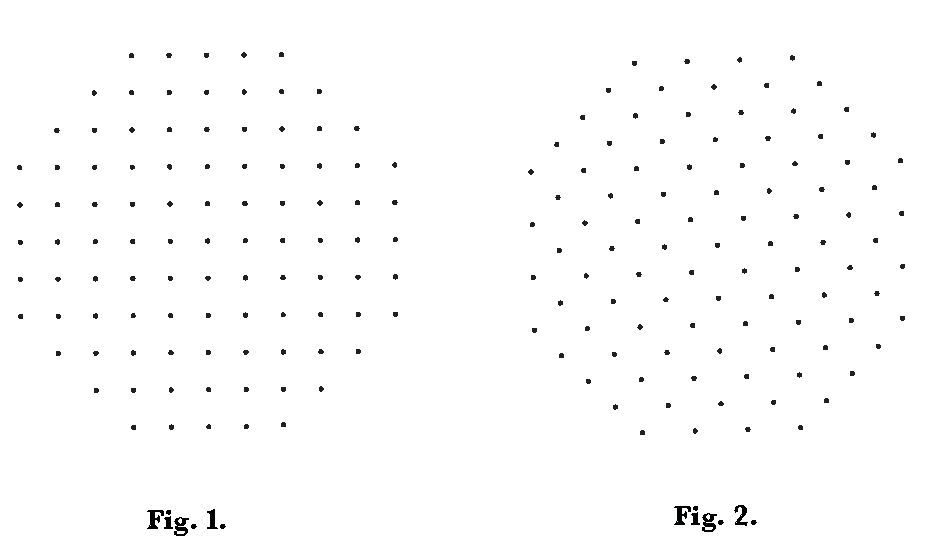
\includegraphics[width=3.6in]{peirce-howto1.pdf}

yet it is conceivable that a man should assert one proposition and deny the other. Such false distinctions do as much harm as the confusion of beliefs really different, and are among the pitfalls of which we ought constantly to beware, especially when we are upon metaphysical ground. One singular deception of this sort, which often occurs, is to mistake the sensation produced by our own unclearness of thought for a character of the object we are thinking. Instead of perceiving that the obscurity is purely subjective, we fancy that we contemplate a quality of the object which is essentially mysterious; and if our conception be afterward presented to us in a clear form we do not recognize it as the same, owing to the absence of the feeling of unintelligibility. So long as this deception lasts, it obviously puts an impassable barrier in the way of perspicuous thinking; so that it equally interests the opponents of rational thought to perpetuate it, and its adherents to guard against it.


Another such deception is to mistake a mere difference in the grammatical construction of two words for a distinction between the ideas they express. In this pedantic age, when the general mob of writers attend so much more to words than to things, this error is common enough. When I just said that thought is an \emph{action,} and that it consists in a \emph{relation,} although a person performs an action but not a relation, which can only be the result of an action, yet there was no inconsistency in what I said, but only a grammatical vagueness. 

From all these sophisms we shall be perfectly safe so long as we reflect that the whole function of thought is to produce habits of action; and that whatever there is connected with a thought, but irrelevant to its purpose, is an accretion to it, but no part of it. If there be a unity among our sensations which has no reference to how we shall act on a given occasion, as when we listen to a piece of music, why we do not call that thinking. To develop its meaning, we have, therefore, simply to determine what habits it produces, for what a thing means is simply what habits it involves. Now, the identity of a habit depends on how it might lead us to act, not merely under such circumstances as are likely to arise, but under such as might possibly occur, no matter how improbable they may be. What the habit is depends on \emph{when} and \emph{how} it causes us to act. As for the \emph{when,} every stimulus to action is derived from perception; as for the \emph{how,} every purpose of action is to produce some sensible result. Thus, we come down to what is tangible and conceivably practical, as the root of every real distinction of thought, no matter how subtile it may be; and there is no distinction of meaning so fine as to consist in anything but a possible difference of practice.


To see what this principle leads to, consider in the light of it such a doctrine as that of transubstantiation. The Protestant churches generally hold that the elements of the sacrament are flesh and blood only in a tropical sense; they nourish our souls as meat and the juice of it would our bodies. But the Catholics maintain that they are literally just meat and blood; although they possess all the sensible qualities of wafercakes and diluted wine. But we can have no conception of wine except what may enter into a belief, either ---
\begin{quote}
1. That this, that, or the other, is wine; or,\\
2. That wine possesses certain properties.
\end{quote}

Such beliefs are nothing but self-notifications that we should, upon occasion, act in regard to such things as we believe to be wine according to the qualities which we believe wine to possess. The occasion  of such action would be some sensible perception, the motive of it to produce some sensible result. Thus our action has exclusive reference to what affects the senses, our habit has the same bearing as our action, our belief the same as our habit, our conception the same as our belief; and we can consequently mean nothing by wine but what has certain effects, direct or indirect, upon our senses; and to talk of something as having all the sensible characters of wine, yet being in reality blood, is senseless jargon. Now, it is not my object to pursue the theological question; and having used it as a logical example I drop it, without caring to anticipate the theologian's reply. I only desire to point out how impossible it is that we should have an idea in our minds which relates to anything but conceived sensible effects of things. Our idea of anything \emph{is} our idea of its sensible effects; and if we fancy that we have any other we deceive ourselves, and mistake a mere sensation accompanying the thought for a part of the thought itself. It is absurd to say that thought has any meaning unrelated to its only function. It is foolish for Catholics and Protestants to fancy themselves in disagreement about the elements of the sacrament, if they agree in regard to all their sensible effects, here and hereafter.
It appears, then, that the rule for attaining the third grade of clearness of apprehension is as follows: Consider what effects, which might conceivably have practical bearings, we conceive the object of our conception to have. Then, our conception of these effects is the whole of our conception of the object.


\subsection*{III}

Let us illustrate this rule by some examples; and, to begin with the simplest one possible, let us ask what we mean by calling a thing \emph{hard}. Evidently that it will not be scratched by many other substances. The whole conception of this quality, as of every other, lies in its conceived effects. There is absolutely no difference between a hard thing and a soft thing so long as they are not brought to the test. Suppose, then, that a diamond could be crystallized in the midst of a cushion of soft cotton, and should remain there until it was finally burned up. Would it be false to say that that diamond was soft? This seems a foolish question, and would be so, in fact, except in the realm of logic. There such questions are often of the greatest utility as serving to bring logical principles into sharper relief than real discussions ever could. In studying logic we must not put them aside with hasty answers, but must consider them with attentive care, in order  to make out the principles involved. We may, in the present case, modify our question, and ask what prevents us from saying that all hard bodies remain perfectly soft until they are touched, when their hardness increases with the pressure until they are scratched. Reflection will show that the reply is this: there would be no \emph{falsity} in such modes of speech. They would involve a modification of our present usage of speech with regard to the words hard and soft, but not of their meanings. For they represent no fact to be different from what it is; only they involve arrangements of facts which would be exceedingly maladroit. This leads us to remark that the question of what would occur under circumstances which do not actually arise is not a question of fact, but only of the most perspicuous arrangement of them. For example, the question of free-will and fate in its simplest form, stripped of verbiage, is something like this: I have done something of which I am ashamed; could I, by an effort of the will, have resisted the temptation, and done otherwise? The philosophical reply is, that this is not a question of fact, but only of the arrangement of facts. Arranging them so as to exhibit what is particularly pertinent to my question--- namely, that I ought to blame myself for having done wrong--- it is perfectly true to say that, if I had willed to do otherwise than I did, I should have done otherwise. On the other hand, arranging the facts so as to exhibit another important consideration, it is equally true that, when a temptation has once been allowed to work, it will, if it has a certain force, produce its effect, let me struggle how I may. There is no objection to a contradiction in what would result from a false supposition. The \emph{reductio ad absurdum} consists in showing that contradictory results would follow from a hypothesis which is consequently judged to be false. Many questions are involved in the free-will discussion, and I am far from desiring to say that both sides are equally right. On the contrary, I am of opinion that one side denies important facts, and that the other does not. But what I do say is, that the above single question was the origin of the whole doubt; that, had it not been for this question, the controversy would never have arisen; and that this question is perfectly solved in the manner which I have indicated. 


Let us next seek a clear idea of Weight. This is another very easy case. To say that a body is heavy means simply that, in the absence of opposing force, it will fall. This (neglecting certain specifications of how it will fall, etc., which exist in the mind of the physicist who uses the word) is evidently the whole conception of weight. It is a fair question whether some particular facts may not \emph{account} for gravity;  but what we mean by the force itself is completely involved in its effects.
 
This leads us to undertake an account of the idea of Force in general. This is the great conception which, developed in the early part of the seventeenth century from the rude idea of a cause, and constantly improved upon since, has shown us how to explain all the changes of motion which bodies experience, and how to think about all physical phenomena; which has given birth to modern science, and changed the face of the globe; and which, aside from its more special uses, has played a principal part in directing the course of modern thought, and in furthering modern social development. It is, therefore, worth some pains to comprehend it. According to our rule, we must begin by asking what is the immediate use of thinking about force; and the answer is, that we thus account for changes of motion. If bodies were left to themselves, without the intervention of forces, every motion would continue unchanged both in velocity and in direction. Furthermore, change of motion never takes place abruptly; if its direction is changed, it is always through a curve without angles; if its velocity alters, it is by degrees. The gradual changes which are constantly taking place are conceived by geometers to be compounded together according to the rules of the parallelogram of forces. If the reader does not already know what this is, he will find it, I hope, to his advantage to endeavor to follow the following explanation; but if mathematics are insupportable to him, pray let him skip three paragraphs rather than that we should part company here.


A \emph{path} is a line whose beginning and end are distinguished. Two paths are considered to be equivalent, which, beginning at the same point, lead to the same point. Thus the two paths, \emph{A B C D E} and \emph{A F G H E,} are equivalent. Paths which do not begin at the same point are considered to be equivalent, provided that, on moving either of them without turning it, but keeping it always parallel to its original position, when its beginning coincides with that of the other path, the ends also coincide. Paths are considered as geometrically added together, when one begins where the other ends; thus the path \emph{A E} is conceived to be a sum of \emph{A B, B C, C D,} and \emph{D E.} In the parallelogram of Fig. 4 the diagonal \emph{A C} is the sum of \emph{A B} and \emph{B C;} or, since \emph{A D} is geometrically equivalent to \emph{B C, A C} is the geometrical sum of \emph{A B} and \emph{A D.}

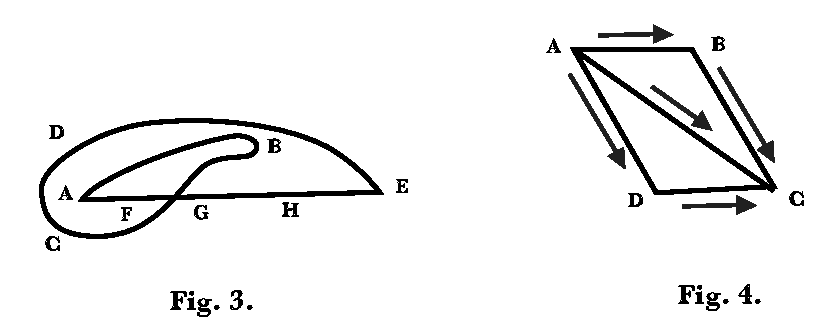
\includegraphics[width=3.6in]{peirce-howto2.pdf}

All this is purely conventional. It simply amounts to this: that we choose to call paths having the relations I have described equal or added. But, though it is a convention, it is a convention with a good reason. The rule for geometrical addition may be applied not only to paths, but to any other things which can be represented by paths. Now, as a path is determined by the varying direction and distance of the point which moves over it from the starting-point, it follows that anything which from its beginning to its end is determined by a varying direction and a varying magnitude is capable of being represented by a line. Accordingly, \emph{velocities} may be represented by lines, for they have only directions and rates. The same thing is true of \emph{accelerations,} or changes of velocities. This is evident enough in the case of velocities; and it becomes evident for accelerations if we consider that precisely what velocities are to positions--- namely, states of change of them--- that accelerations are to velocities.


The so-called ``parallelogram of forces'' is simply a rule for compounding accelerations. The rule is, to represent the accelerations by paths, and then to geometrically add the paths. The geometers, however, not only use the ``parallelogram of forces'' to compound different accelerations, but also to resolve one acceleration into a sum of several. Let \emph{A B} (Fig. 5) be the path which represents a certain acceleration--- say, such a change in the motion of a body that at the end of one second the body will, under the influence of that change, be in a position different from what it would have had if its motion had  continued unchanged such that a path equivalent to \emph{A B} would lead from the latter position to the former. This acceleration may be considered as the sum of the accelerations represented by \emph{A C} and \emph{C B.} It may also be considered as the sum of the very different accelerations represented by \emph{A D} and \emph{D B,} where \emph{A D} is almost the opposite of \emph{A C.} And it is clear that there is an immense variety of ways in which \emph{A B} might be resolved into the sum of two accelerations.

\centerline{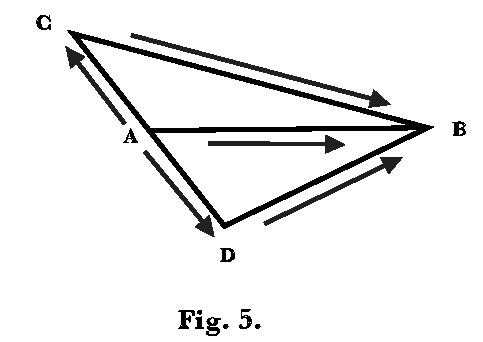
\includegraphics[width=1.6in]{peirce-howto3.pdf}}

After this tedious explanation, which I hope, in view of the extraordinary interest of the conception of force, may not have exhausted the reader's patience, we are prepared at last to state the grand fact which this conception embodies. This fact is that if the actual changes of motion which the different particles of bodies experience are each resolved in its appropriate way, each component acceleration is precisely such as is prescribed by a certain law of Nature, according to which bodies in the relative positions which the bodies in question actually have at the moment\authornote{Possibly the velocities also have to be taken into account.} always receive certain accelerations, which, being compounded by geometrical addition, give the acceleration which the body actually experiences.


This is the only fact which the idea of force represents, and whoever will take the trouble clearly to apprehend what this fact is, perfectly comprehends what force is. Whether we ought to say that a force \emph{is} an acceleration, or that it \emph{causes} an acceleration, is a mere question of propriety of language, which has no more to do with our real meaning than the difference between the French idiom ``\emph{Il fait froid}'' and its English equivalent ``\emph{It is cold}.'' Yet it is surprising to see how this simple affair has muddled men's minds. In how many profound treatises is not force spoken of as a ``mysterious entity,'' which seems to be only a way of confessing that the author despairs of ever getting a clear notion of what the word means! In a recent admired work on Analytic Mechanics it is stated that we understand precisely the effect of force, but what force itself is we do not understand! This is simply a self-contradiction. The idea which the word force excites in our minds has no other function than to affect our actions, and these actions can have no reference to force otherwise than through its effects. Consequently, if we know what the effects of force are, we are acquainted with every fact which is implied in saying that a force exists, and there is nothing more to know. The truth is, there is some vague notion afloat that a question may  mean something which the mind cannot conceive; and when some hair-splitting philosophers have been confronted with the absurdity of such a view, they have invented an empty distinction between positive and negative conceptions, in the attempt to give their non-idea a form not obviously nonsensical. The nullity of it is sufficiently plain from the considerations given a few pages back; and, apart from those considerations, the quibbling character of the distinction must have struck every mind accustomed to real thinking.

\subsection*{IV}



Let us now approach the subject of logic, and consider a conception which particularly concerns it, that of \emph{reality.} Taking clearness in the sense of familiarity, no idea could be clearer than this. Every child uses it with perfect confidence, never dreaming that he does not understand it. As for clearness in its second grade, however, it would probably puzzle most men, even among those of a reflective turn of mind, to give an abstract definition of the real. Yet such a definition may perhaps be reached by considering the points of difference between reality and its opposite, fiction. A figment is a product of somebody's imagination; it has such characters as his thought impresses upon it. That those characters are independent of how you or I think is an external reality. There are, however, phenomena within our own minds, dependent upon our thought, which are at the same time real in the sense that we really think them. But though their characters depend on how we think, they do not depend on what we think those characters to be. Thus, a dream has a real existence as a mental phenomenon, if somebody has really dreamt it; that he dreamt so and so, does not depend on what anybody thinks was dreamt, but is completely independent of all opinion on the subject. On the other hand, considering, not the fact of dreaming, but the thing dreamt, it retains its peculiarities by virtue of no other fact than that it was dreamt to possess them. Thus we may define the real as that whose characters are independent of what anybody may think them to be. 
 
But, however satisfactory such a definition may be found, it would be a great mistake to suppose that it makes the idea of reality perfectly clear. Here, then, let us apply our rules. According to them, reality, like every other quality, consists in the peculiar sensible effects which things partaking of it produce. The only effect which real things have is to cause belief, for all the sensations which they excite emerge into  consciousness in the form of beliefs. The question therefore is, how is true belief (or belief in the real) distinguished from false belief (or belief in fiction). Now, as we have seen in the former paper, the ideas of truth and falsehood, in their full development, appertain exclusively to the experiential method of settling opinion. A person who arbitrarily chooses the propositions which he will adopt can use the word truth only to emphasize the expression of his determination to hold on to his choice. Of course, the method of tenacity never prevailed exclusively; reason is too natural to men for that. But in the literature of the dark ages we find some fine examples of it. When Scotus Erigena is commenting upon a poetical passage in which hellebore is spoken of as having caused the death of Socrates, he does not
hesitate to inform the inquiring reader that Helleborus and Socrates were two eminent Greek philosophers, and that the latter, having been overcome in argument by the former, took the matter to heart and died of it! What sort of an idea of truth could a man have who could adopt and teach, without the qualification of a perhaps, an opinion taken so entirely at random? The real spirit of Socrates, who I hope would have been delighted to have been ``overcome in argument,'' because he would have learned something by it, is in curious contrast with the naive idea of the glossist, for whom discussion would seem to have been simply a struggle. When philosophy began to awake from its long slumber, and before theology completely dominated it, the practice seems to have been for each professor to seize upon any philosophical position he found unoccupied and which seemed a strong one, to intrench himself in it, and to sally forth from time to time to give battle to the others. Thus, even the scanty records we possess of those disputes enable us to make out a dozen or more opinions held by different teachers at one time concerning the question of nominalism and realism. Read the opening part of the ``Historia Calamitatum'' of Abelard, who was certainly as philosophical as any of his contemporaries, and see the spirit of
combat which it breathes. For him, the truth is simply his particular stronghold. When the method of authority prevailed, the truth meant little more than the Catholic faith. All the efforts of the scholastic doctors are directed toward harmonizing their faith in Aristotle and their faith in the Church, and one may search their ponderous folios through without finding an argument which goes any further. It is noticeable that where different faiths flourish side by side, renegades are looked upon with contempt even by the party whose belief they adopt; so completely has the idea of loyalty replaced that of truth-seeking. Since the  time of Descartes, the defect in the conception of truth has been less apparent. Still, it will sometimes strike a scientific man that the philosophers have been less intent on finding out what the facts are, than on inquiring what belief is most in harmony with their system. It is hard to convince a follower of the \emph{a priori} method by adducing facts; but show him that an opinion he is defending is inconsistent with what he has laid down elsewhere, and he will be very apt to retract it. These minds do not seem to believe that disputation is ever to cease; they seem to think that the opinion which is natural for one man is not so for another, and that belief will, consequently, never be settled. In contenting themselves with fixing their own opinions by a method which would lead another man to a different result, they betray their feeble hold of the conception of what truth is. 

On the other hand, all the followers of science are animated by a cheerful hope that the processes of investigation, if only pushed far enough, will give one certain solution to each question to which they can be applied. One man may investigate the velocity of light by studying the
transits of Venus and the aberration of the stars; another by the oppositions of Mars and the eclipses of Jupiter's satellites; a third by the method of Fizeau; a fourth by that of Foucault; a fifth by the motions of the curves of
Lissajoux; a sixth, a seventh, an eighth, and a ninth, may follow the different methods of comparing the measures of statical and dynamical electricity. They may at first obtain different results, but, as each perfects his method and his processes, the results are found to move steadily together toward a destined center. So with all scientific research. Different minds may set out with the most antagonistic views, but the progress of investigation carries them by a force outside of themselves to one and the same conclusion. This activity of thought by which we are carried, not where we wish, but to a fore-ordained goal, is like the operation of destiny. No modification of the
point of view taken, no selection of other facts for study, no natural bent of mind even, can enable a man to escape the predestinate opinion. This great law is embodied in the conception of truth and reality. The opinion which is fated\authornote{Fate means merely that which is sure to come true, and can nohow be avoided. It is a superstition to suppose that a certain sort of events are ever fated, and it is another to suppose that the word fate can never be freed from its superstitious taint. We are all fated to die.} to be ultimately agreed to by all who investigate, is what we mean by the truth, and the object represented in this opinion is the real. That is the way I would explain reality.


But it may be said that this view is directly opposed to the abstract  definition which we have given of reality, inasmuch as it makes the characters of the real depend on what is ultimately thought about them. But the answer to this is that, on the one hand, reality is independent, not necessarily of thought in general, but only of what you or I or any finite number of men may think about it; and that, on the other hand, though the
object of the final opinion depends on what that opinion is, yet what that opinion is does not depend on what you or I or any man thinks. Our perversity and that of others may indefinitely postpone the settlement of opinion; it
might even conceivably cause an arbitrary proposition to be universally accepted as long as the human race should last. Yet even that would not change the nature of the belief, which alone could be the result of investigation
carried sufficiently far; and if, after the extinction of our race, another should arise with faculties and disposition for investigation, that true opinion must be the one which they would ultimately come to. ``Truth crushed to
earth shall rise again,'' and the opinion which would finally result from investigation does not depend on how anybody may actually think. But the reality of that which is real does depend on the real fact that investigation
is destined to lead, at last, if continued long enough, to a belief in it. 



But I may be asked what I have to say to all the minute facts of history, forgotten never to be recovered, to the lost books of the ancients, to the buried secrets.
\begin{quote}
Full many a gem of purest ray serene\\
The dark, unfathomed caves of ocean bear;\\
Full many a flower is born to blush unseen,\\
And waste its sweetness on the desert air.
\end{quote}
Do these things not really exist because they are hopelessly beyond the reach of our knowledge? And then, after the universe is dead (according to the prediction of some scientists), and all life has ceased forever, will not the shock of atoms continue though there will be no mind to know it? To this I reply that, though in no possible state of knowledge can any number be great enough to express the relation between the amount of what rests unknown to the amount of the known, yet it is unphilosophical to suppose that, with regard to any given question (which has any clear meaning), investigation would not bring forth a solution of it, if it were carried far enough. Who would have said, a few years ago, that we could ever know of what substances stars are made whose light may have been longer in reaching us than the human race has existed? Who can be sure of  what we shall not know in a few hundred years? Who can guess what would be the result of continuing the pursuit of science for ten thousand years, with the activity of the last hundred? And if it were to go on for a million, or a billion, or any number of years you please, how is it possible to say that there is any question which might not ultimately be solved?


But it may be objected, ``Why make so much of these remote considerations, especially when it is your principle that only practical distinctions have a meaning?'' Well, I must confess that it makes very little difference whether we say that a stone on the bottom of the ocean, in complete darkness, is brilliant or not--- that is to say, that it
\emph{probably} makes no difference, remembering always that stone \emph{may} be fished up tomorrow. But that there are gems at the bottom of the sea, flowers in the untraveled desert, etc., are propositions which,  like that about a diamond being hard when it is not pressed, concern much more the arrangement of our language than they do the meaning of our ideas. 

It seems to me, however, that we have, by the
application of our rule, reached so clear an apprehension of what we mean by reality, and of the fact which the idea rests on, that we should not, perhaps, be making a pretension so presumptuous as it would be singular, if we were to
offer a metaphysical theory of existence for universal acceptance among those who employ the scientific method of fixing belief. However, as metaphysics is a subject much more curious than useful, the knowledge of which, like that of a sunken reef, serves chiefly to enable us to keep clear of it, I will not trouble the reader with any more Ontology at this moment. I have already been led much further into that path than I should have desired; and I have given the reader such a dose of mathematics, psychology, and all that is most abstruse, that I fear he may already have left me, and that what I am now writing is for the compositor and proof-reader exclusively. I trusted to the
importance of the subject. There is no royal road to logic, and really valuable ideas can only be had at the price of close attention. But I know that in the matter of ideas the public prefer the cheap and nasty; and in my next paper I am going to return to the easily intelligible, and not wander from it again. The reader who has been at the pains of wading through this paper, shall be rewarded in the next one by seeing how beautifully what has been developed in this tedious way can be applied to the ascertainment of the rules of scientific reasoning.


We have, hitherto, not crossed the threshold of scientific logic. It  is certainly important to know how to make our ideas clear, but they may be ever so clear without being true. How to make them so, we have next to study. How to give birth to those vital and procreative ideas which multiply into a thousand forms and diffuse themselves everywhere, advancing civilization and making the dignity of man, is an art not yet reduced to rules, but of the secret of which the history of science affords some hints.


